\Chapter{Kivételes esetek}
Sajnálatos módon az indikátorokkal történő kereskedés sem jelent 100\%-os hozamot, hiszen nem tud minden tényezővel számolni az algoritmus. Az indikátorok jellemzően késnek, hamarabb következik be a változás, mint az indikátor jelzése. Ebben a fejezetben szeretnék bemutatni néhány tényezőt grafikonokkal, amelyek megnehezítik az automata dolgát.

\Section{GameStop short squeeze}
A GameStop egy elavult üzleti modellel bíró, csökkenő árbevételt elérő vállalat. Ennek az a magyarázata, hogy boltokban értékesítenek számítógépes játékokat, holott már a platformok nagy része online adja el őket. Ez volt az oka annak, hogy elég sokan sholtolták a céget, hiszen egyre többen bíztak abban, hogy csődközeli állapotba fog térni a vállalat. Azonban egy internetes közösségi oldalon, a Redditen lévő felhasználók short squeeze-t váltottak ki. A csúcspontján, január 28-án a részvényeinek árfolyama 500\$ fölött jártak, ami a hónap eleji 17\$-hoz képest 30-szoros emelkedés.
\begin{figure}[ht]
\centering
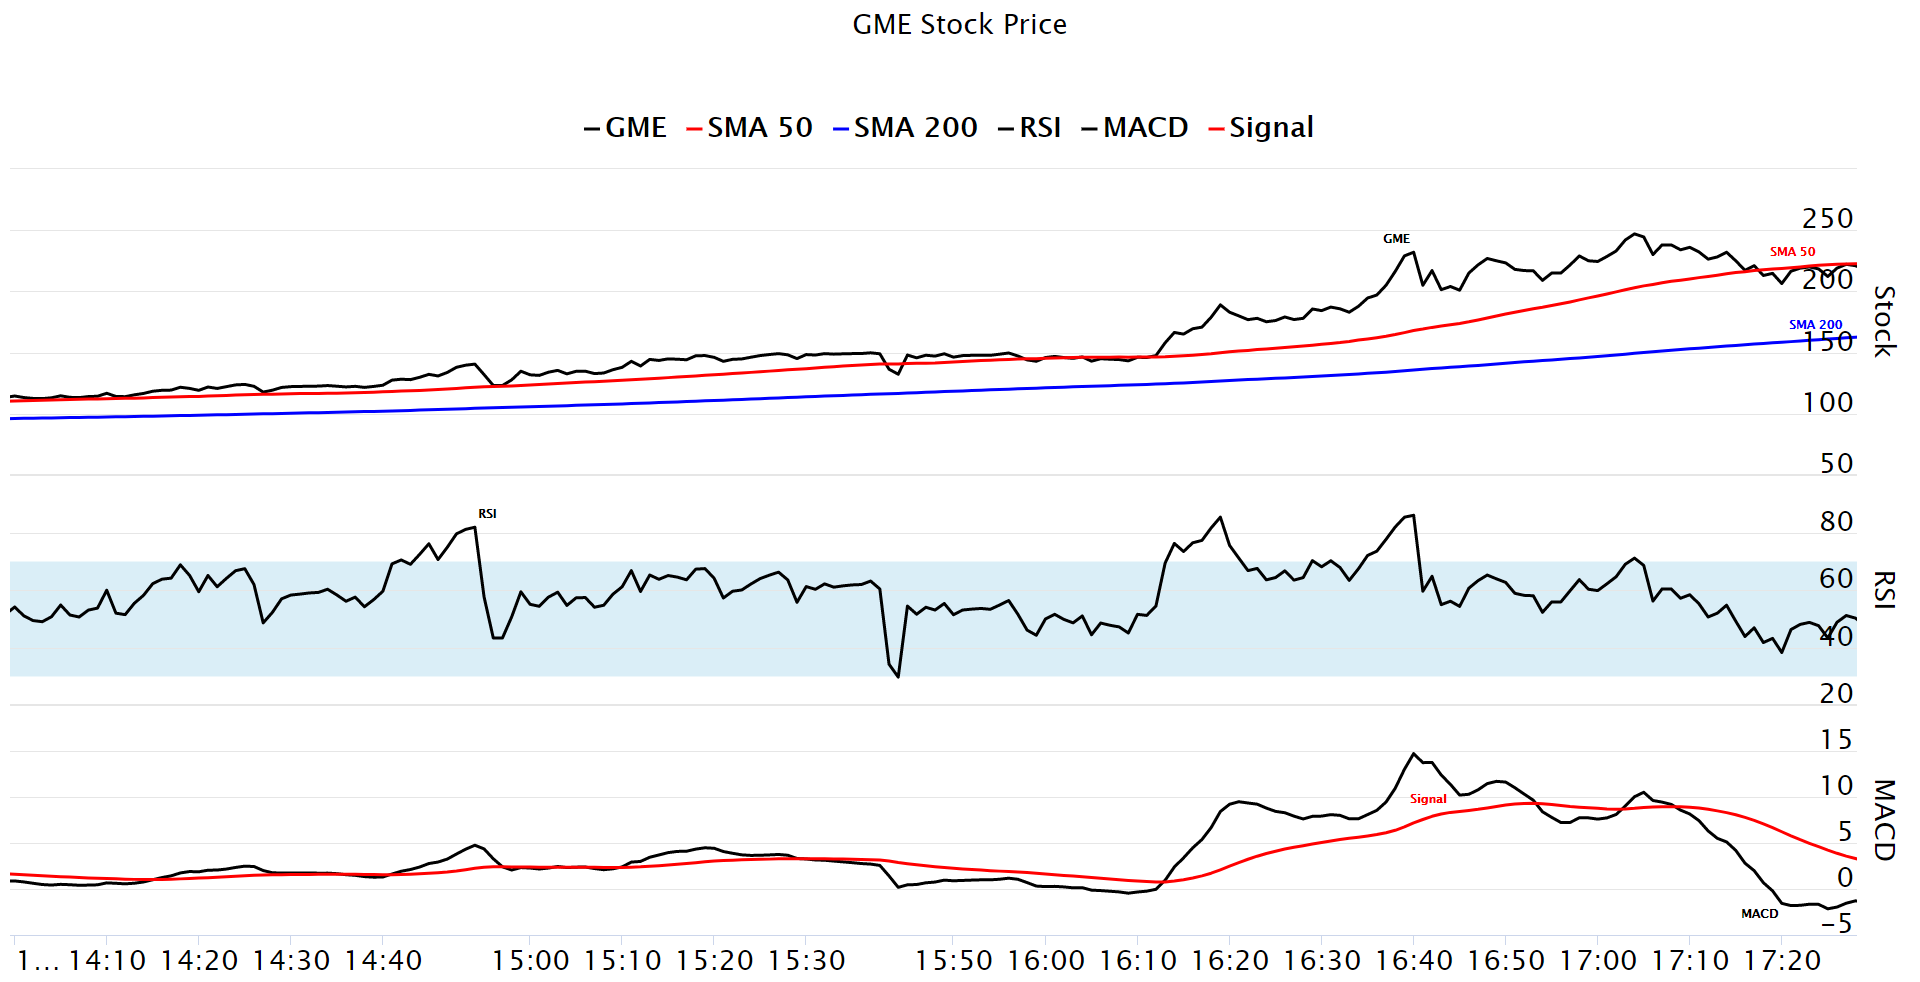
\includegraphics[width=\textwidth]{images/GME_sq.png}
\caption{GameStop részvény short squeeze közben.}
\label{fig:GME_sq}
\end{figure}
Látható az ábrán, hogy az indikátorok milyen meredeken kezdtek el emelkedni, az MACD is korábban nem látott magasságokba ugrott. Az indikátorok közül az MACD jelzi egyedül, hogy vásárolni kellene, azonban 27\$-t ugrott már mire az indikátor bejelzett.

\Section{Hírérzékenység}
Az internet fejlődése lehetővé tette a hírek gyors terjedését, ezért manapság egy cégtulajdonos, ha negatív hírt tesz közzé az üzenőfalán, akkor nagyon megmozdulhat az árfolyama a cégének. Például a Tesla vezetője Elon Musk a kedvenc social media platformjára, a Twitterre május elsején kiírta, hogy szerinte túl magas a Tesla árfolyama. Erre reagálva a befektetők adták el a részvényeiket amíg tudták, és egy óra alatt majdnem 15\$-os különbséget generáltak.
\begin{figure}[ht]
\centering
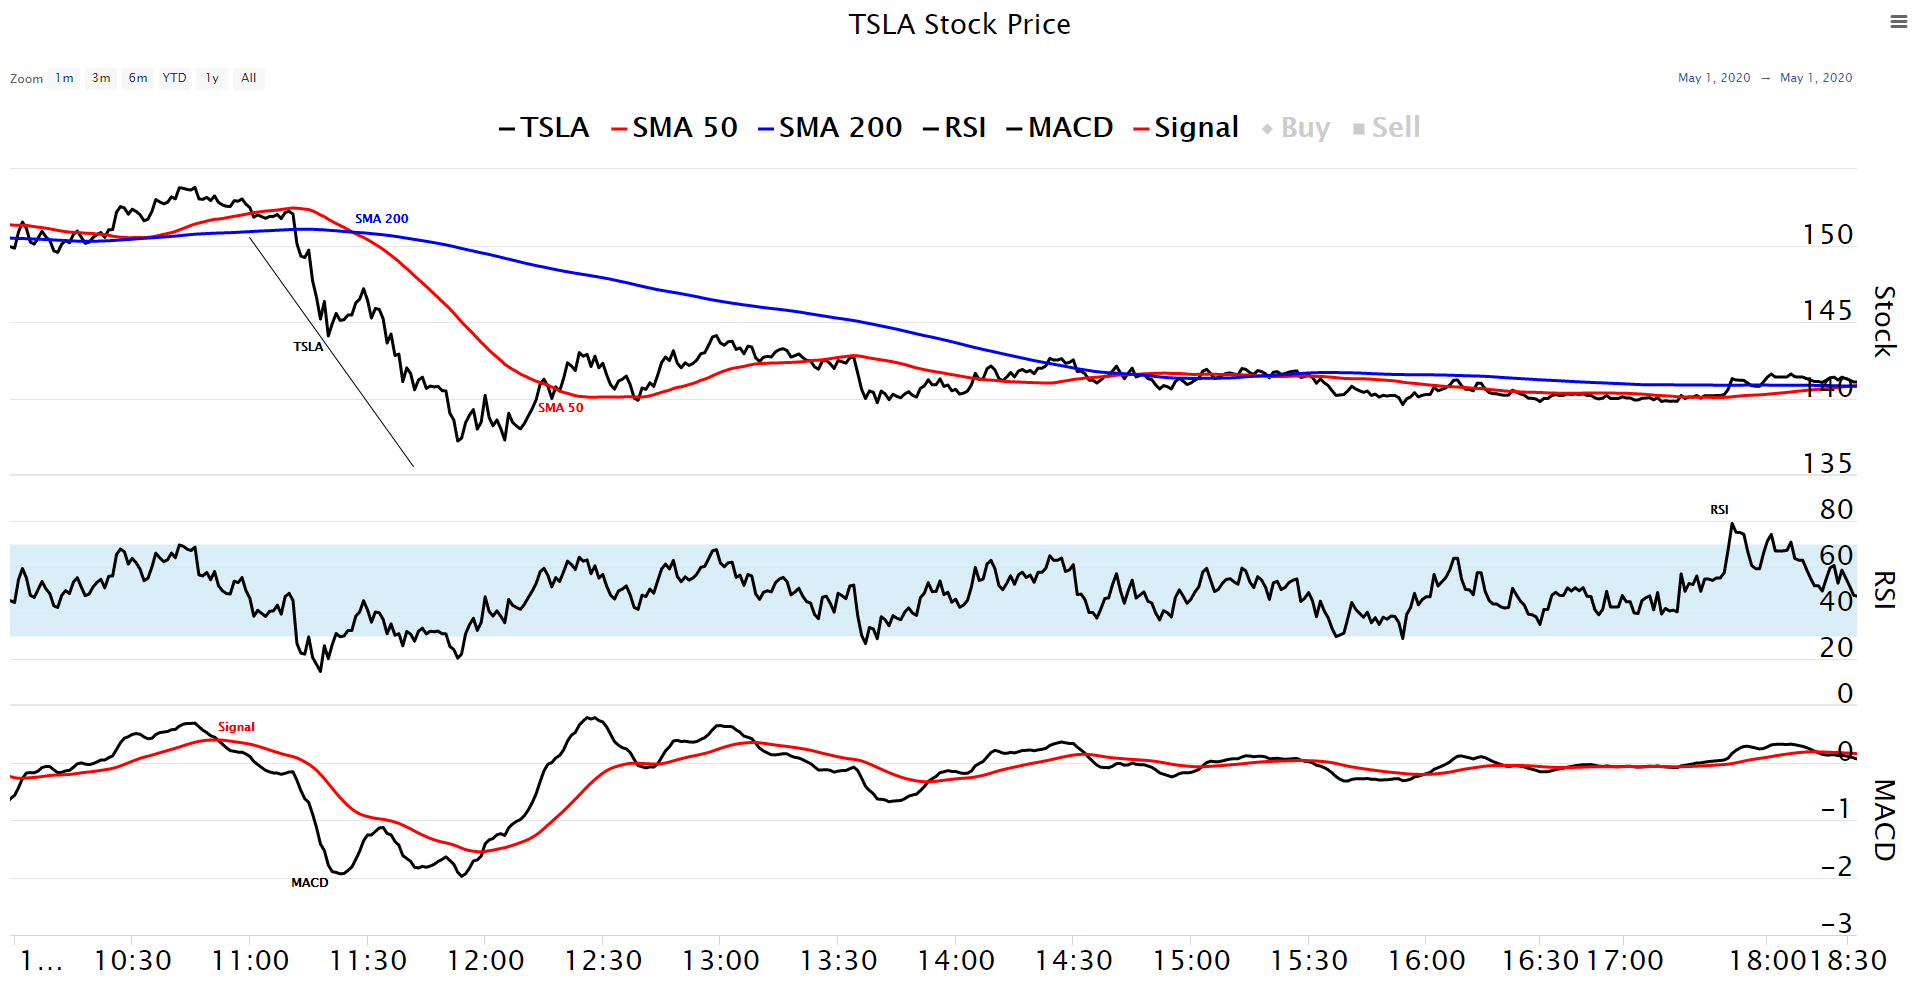
\includegraphics[width=\textwidth]{images/TSLA_news.png}
\caption{A Tesla részvény esése egy megjelent vélemény miatt.}
\label{fig:TSLA_news}
\end{figure}



%short squeeze: gamestop
%https://en.wikipedia.org/wiki/GameStop_short_squeeze

%hírérzékenység: TSLA 04.18.
%https://www.theguardian.com/technology/2021/apr/19/two-die-in-tesla-crash-no-one-in-drivers-seat-police
%kis adatmennyiség

%világjárvány 